\section{Description of the chosen DSP}\label{sec:dsp_description}


The chosen \gls{dsp} is the Texas Instruments TMS320C5515 Fixed-Point Digital Signal Processor.
The \gls{dsp} can perform at four different clock rates, dependent on the supply voltage. It can run \SI{60}{\mega\hertz} or \SI{75}{\mega\hertz}, if the supply voltage is \SI{1.05}{\volt}, giving cycle times of \SI{16.67}{\nano\second} or \SI{13.3}{\nano\second}. If the supply voltage is \SI{1.3}{\volt} the \gls{dsp} can run a \SI{100}{\mega\hertz}- or \SI{120}{\mega\hertz}- clock, giving cycle times of \SI{10}{\nano\second} or \SI{8.33}{\nano\second}. The \gls{dsp} can do one/two instructions per cycle. An example of when the \gls{dsp} can do two instructions per cycle, is when a multiplication and an addition is done. The \gls{dsp} has two \gls{mac}'s, making it able to do one 17-bit times 17-bit multiplication and one 32-bit addition in one cycle. This means the \gls{dsp} can do potentially $2 \cdot 120 \cdot 10^6 = 240$ \gls{mips}. The \gls{dsp} has a 8 to 1024 point 16-bit \gls{fft} hardware accelerator, and supports \gls{uart}, \gls{spi}, \gls{i2c} and \gls{i2s} communication protocols \citep{c5515}.
\subsection{Memory on the DSP}
\begin{figure}[h]
	\centering
		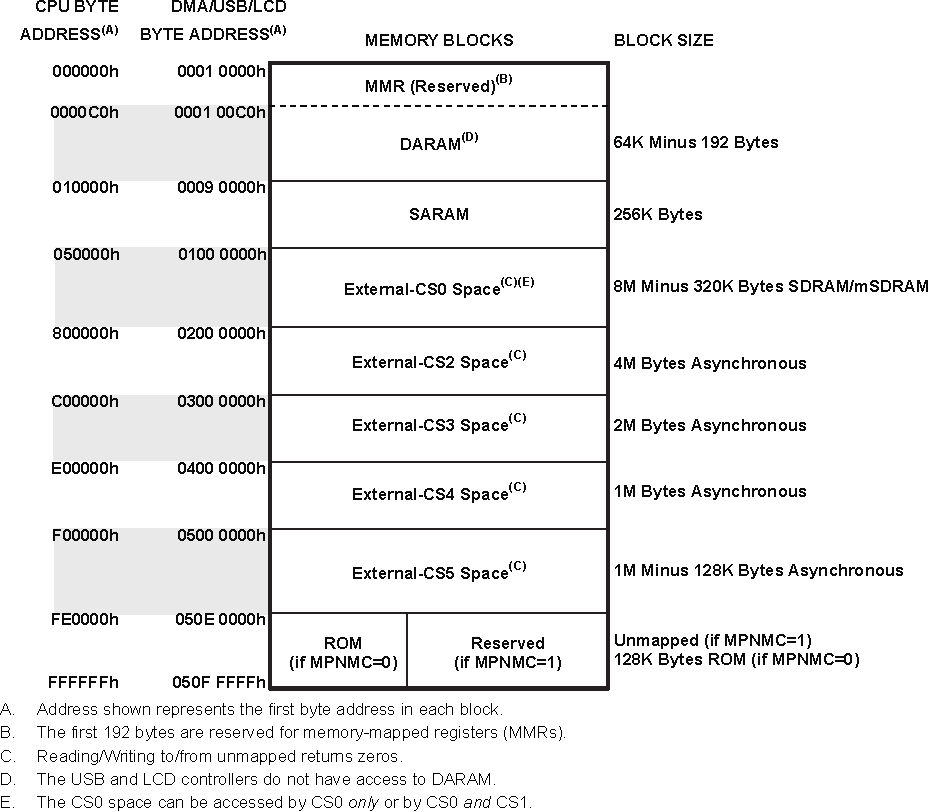
\includegraphics[width=1\textwidth]{memory_dsp.pdf}
		\caption{The figure shows the memory map of the TMS320C5515.}
		\label{fig:dps_memory}
\end{figure}
The \gls{dsp} has \SI{448}{\kilo\byte} on-chip memory divided in \SI{320}{\kilo\byte} \gls{ram} and \SI{128}{\kilo\byte} \gls{rom}. The \gls{ram} is divided in \SI{256}{\kilo\byte} \gls{saram} and \SI{64}{\kilo\byte} \gls{daram}, while all the \gls{rom} is \gls{sarom}.
The \gls{daram} is divided into eight blocks of 4K words, which each can do two instructions per cycle. The \gls{daram} is located in the memory addresses from 000000h to 00FFFFh. The \gls{saram} is divided into 32 blocks of 4K words, which each can do one instruction per cycle. The \gls{saram} is located in the memory addresses from 010000h to 04FFFFh. The \gls{sarom} is divided in four 16K word blocks, where there in each block can be accessed one word per cycle. The \gls{sarom} is located in the addresses from FE0000h to FFFFFFh \cite{c5515}. The placement of the memory is illustrated in \autoref{fig:dps_memory}.
\subsection{The CPU}
The \gls{cpu} on the chosen \gls{dsp} is based on the C55x CPU 3.3 generation processor core. The \gls{cpu} was described a bit in the introduction of the \gls{dsp}, but some further explanation will be made here. The \gls{cpu} has an internal bus structure with one program bus, three data read buses and two data write buses. Further more it has additional buses for peripheral and \gls{dma} activities. The data read buses consists of one 32-bit bus and two 16-bit buses, while the two data write buses are both 16-bit. This bus structure makes the \gls{dsp} able to make up to four data reads and two data writes in one cycle. Independent and in parallel of the \gls{cpu}, one 32-bit data transfer can be done per cycle, by each \gls{dma} controller. The \gls{cpu} has both a central 40-bit \gls{alu} and an additional 16-bit \gls{alu}, for operations such as adding, incrementing, bitwise logical operations and bit shift operations. 
The \gls{cpu} uses fully protected pipelining to avoiding conflicts in either fetching or execution, by inserting inactive cycles between instructions that would conflict \citep{c55x_cpu}.
A diagram of the \gls{cpu}'s architecture, including both data- and address- buses and units in the \gls{cpu}, is shown in \autoref{fig:c55x_CPU}.

\begin{figure}[!h]
    \centering
        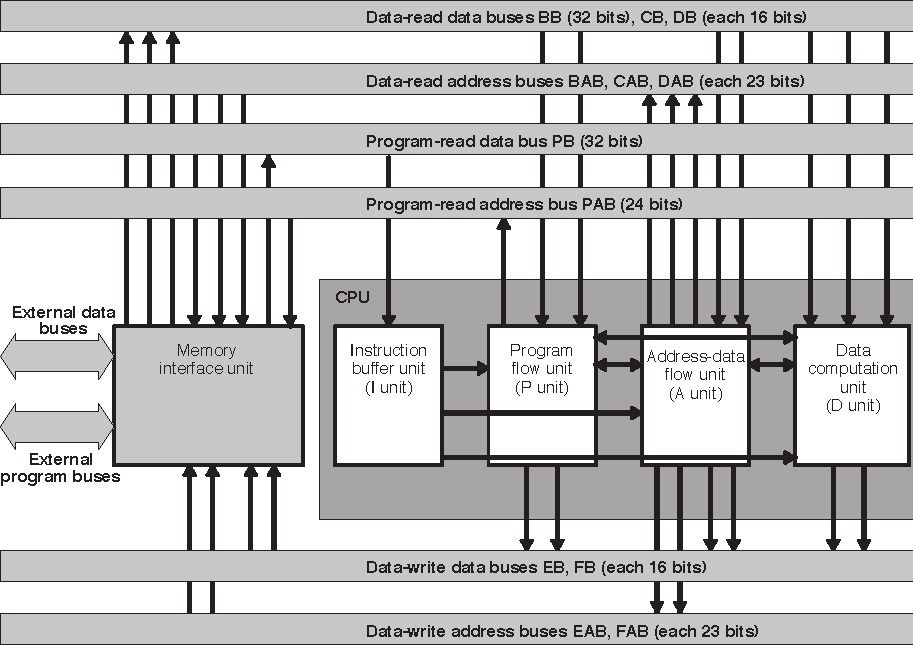
\includegraphics[width=1\textwidth]{c55x_cpu.pdf}
        \caption{Diagram of TMS320C55x CPU architecture \citep{c55x_cpu}.}
        \label{fig:c55x_CPU}
  \end{figure}  
  
\subsection{Registers in the DSP}
Knowledge of the registers are important when programming a \gls{dsp}, if it is chosen to program it in assembly and not in C. The different registers are assigned to do specific tasks and thereby the programmer has to know which registers should be used for which tasks. The TMS320C5515 has e.g four accumulator registers called AC0-AC3. An accumulator register assists with data computation in the \gls{alu}, the \gls{mac}'s and the shifter, meaning if it is wanted to add two numbers, this can be done in an accumulator register. 
Another example is the three registers BK03, BK47 and BKC, which are all circular buffer size registers. Each of these registers sets the number of words in a circular buffer (at max 65535) \citep{c55x_cpu}.  

\subsection{The TMS320C5515 eZdsp development board}
The TMS320C5515 is placed on a developmentboard called TMS320C5515 eZdsp. Some of the boards key features are shown in \autoref{fig:ezdsp}.

\begin{figure}[!h]
    \centering
        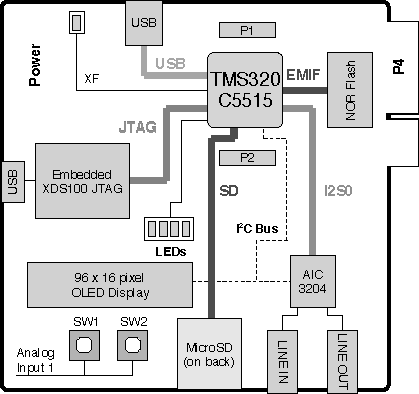
\includegraphics[width=0.8\textwidth]{ezdsp.pdf}
        \caption{Diagram the eZdsp board \citep{ezdsp}.}
        \label{fig:ezdsp}
  \end{figure}

\autoref{fig:ezdsp} shows that the board contains several features such as NOR flash memory, JTAG interface for debugging, an OLED display and a TLV320AIC3204 converter \citep{ezdsp}.  
The converter contains a stereo \gls{adc} with a dynamic range of \SI{92}{\decibel} (16-bit) and with a \gls{snr} of \SI{93}{\decibel}, and a stereo \gls{dac} with a dynamic range of \SI{100}{\decibel} (17-bit) and with a \gls{snr} of \SI{100}{\decibel}. Both the \gls{adc} and the \gls{dac} can run at sampling rates from \SI{8}{\kilo\hertz} to \SI{192}{\kilo\hertz} \citep{TLV320AIC3204}.

%
%\subsection{Power}
%
%The DSP processor gets its power from the \gls{usb} connection.
%
%\subsection{Different Ports}
%
%The C5515 features multiple ports and connectors. It has a micro SD connector, an expansion edge connector as well as a two \gls{usb}s. It also has an audio IN and two Bluetooth interfaces. \\
%
%Each USB connector has a different role, one is used for software purposes and the other one to connect to the personal computer. 
%
%\subsection{LCD Screen}
%
%The \gls{dsp} processor has also an LCD screen that can print different characters by using a string of 14 pins. 
%
%\subsection{Interface with the User}
%
%The processor contains two switch buttons that can be integrated in the software to create an action. 
%
%\subsection{Expansion}
%
%The expansion connectors can be used to redirect the signals to other user interfaces that can be attached to some of the pins on the DSP. The exact number of the pins is in the data sheet. 
%
%\subsection{Monitoring and Testing}
%
%Several "Test points" are available in order to see the signals' behavior moving in the \gls{dsp} processor.
%
%\subsection{Performance}
%
%The \gls{dsp} can run on different speeds depending on how much the \gls{cpu} is powered. The clock rate can be between 60 and 75 MHz if powered with 1.05 Volts and between 100 and 120 MHz if powered with 1.3 Volts. \\
%
%\subsection{Memory}
%
%The chosen DSP has 320 \gls{kb} of \gls{ram} and 128 \gls{kb} of \gls{rom}. \\
%The \gls{ram} consists of a 64 \gls{kb} of dual-access \gls{ram}, 256 \gls{kb} single-access \gls{ram} which clearly gives 320 \gls{kb}. \\
%Dual-access and single access \gls{ram}s presented above can be accessed using an internal program, data or \gls{dma} buses. \\
%Dual-access and single access \gls{ram}s are divided into blocks that can be accessed using byte address ranges. Ranges are defined for each block but all blocks of a same memory type can be regrouped into one address range. \\
%\gls{dma} address range for the block 0 of the dual-access \gls{ram} is 0001 0000h – 0001 1FFFh for instance. \\
%All of the addresses are presented in the data sheet tables 2-2, 2-3.
%The single-access \gls{rom} is also divided into blocks and has an address range. The usable range can be changed using a software. \\
%
%The external memory interface permits a connection to other memories from other devices than the \gls{dsp}. 